\documentclass[10pt]{llncs}

% obsługa języka polskiego
\usepackage[polish]{babel}	% pakiet niezbędny do obsługi języka polskiego
\usepackage[utf8]{inputenc}	% kodowanie dokumentu
\usepackage[T1]{fontenc}	% system kodowania czcionek
\usepackage{polski}		% słownik łamania wyrazów języka polskiego
\usepackage{indentfirst}	% wcięcie w każdym akapicie (polski standard drukarski)
\frenchspacing			% francuskie zwyczaje typograficzne (używane w Polsce)
\usepackage[pdftex]{graphicx}

% kolory
\usepackage[table]{xcolor}

% zapobieganie uciekaniu obrazów na następne strony (metoda \FloatBarrier)
\usepackage[section,subsection,subsubsection]{extraplaceins}

% algorytmy pisane w pseudokodzie
\usepackage{algpseudocode}
\usepackage{algorithm}
\usepackage{amsmath}

% typ czcionki
\usepackage{times}

% numerowanie stron
\pagestyle{headings}

\begin{document}
	
\title{Segmentacja przez progowanie (algorytmem Otsu) i przez klasteryzację (algorytmem ML-EM)}
\author{Maciej Górnicki, Bartosz Stalewski, Rafał Wojdowski}
\institute{CPOO, Dokumentacja projektu}
\maketitle

\section{Temat projektu}

Projekt polegał na zaimplementowaniu dwóch algorytmów służących do segmentacji obrazów na obszary:
\begin{itemize}
	\item algorytmu Otsu, wykonującego segmentację przez progowanie,
	\item algorytmu ML-EM (ang. Maximum Likelihood Estimation Maximization), wykonującego segmentację przez klasteryzację. 
\end{itemize}

\section{Testy algorytmu Otsu}

\subsection{Test algorytmu Otsu --- wybór jednego progu przy histogramie z dwoma skupiskami}

\FloatBarrier

\begin{figure}[h!]
  \centering
  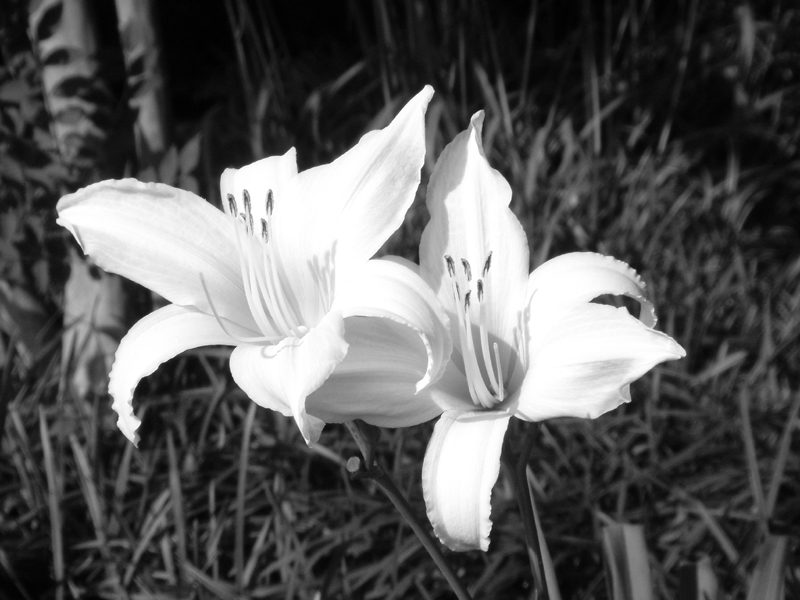
\includegraphics[scale=.3, clip]{img/01.jpg}
	\caption[]
  {Rysunek wejściowy, przedstawiający na pierwszym planie kwiat.}
\end{figure}

\FloatBarrier

\begin{figure}[h!]
  \centering
  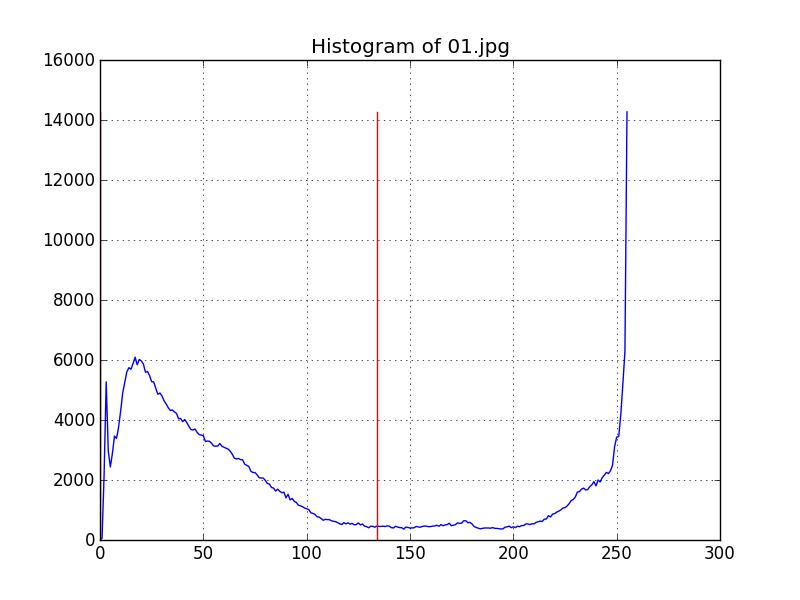
\includegraphics[scale=.3, clip]{img/01_histogram.jpg}
	\caption[]
  {Histogram rysunku wejściowego z zaznaczonym progiem, który został dobrany przez algorytm Otsu. Jak widać, próg został dobrany dość dobrze, ponieważ znajduje się na środku pomiędzy skupiskiem jasnych pikseli (pikseli pierwszego planu) i skupiskiem ciemnych pikseli (pikseli tła).}
\end{figure}

\FloatBarrier

\begin{figure}[h!]
  \centering
  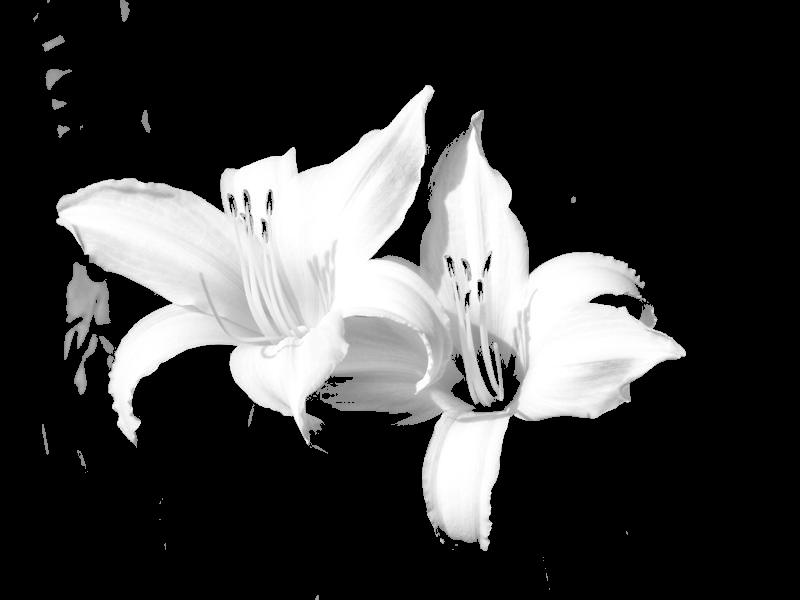
\includegraphics[scale=.3, clip]{img/01_region_01.jpg}
	\caption[]
  {Region pierwszy (z dwóch) po segmentacji.}
\end{figure}

\FloatBarrier

\begin{figure}[h!]
  \centering
  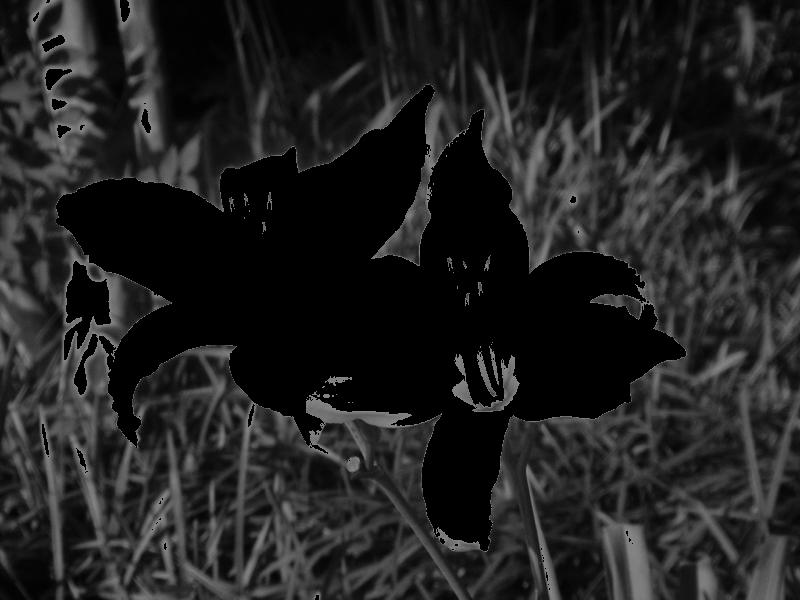
\includegraphics[scale=.3, clip]{img/01_region_02.jpg}
	\caption[]
  {Region drugi (z dwóch) po segmentacji.}
\end{figure}

\FloatBarrier

\subsection{Test algorytmu Otsu --- wybór czterech progów przy histogramie z siedmioma skupiskami}

\FloatBarrier

\begin{figure}[h!]
  \centering
  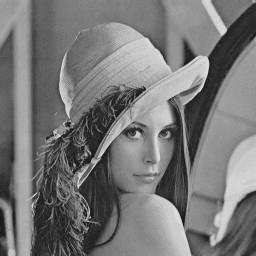
\includegraphics[scale=.8, clip]{img/02.jpg}
	\caption[]
  {Rysunek wejściowy, przedstawiający na pierwszym planie postać.}
\end{figure}

\FloatBarrier

\begin{figure}[h!]
  \centering
  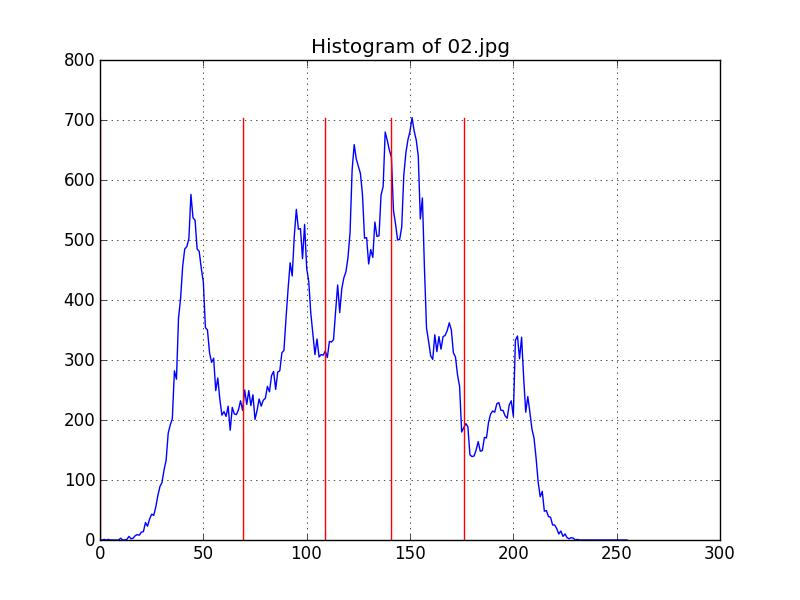
\includegraphics[scale=.3, clip]{img/02_histogram.jpg}
	\caption[]
  {Histogram rysunku wejściowego z zaznaczonymi czteroma progami, które zostały dobrane przez algorytm Otsu. Jak widać, progi zostały dobrane dość dobrze, ponieważ --- po pierwsze --- znajdują się mniej więcej na środku pomiędzy skupiskami i --- po drugie --- są od siebie oddalone w mniej więcej równych odstępach.}
\end{figure}

\FloatBarrier

\begin{figure}[h!]
  \centering
  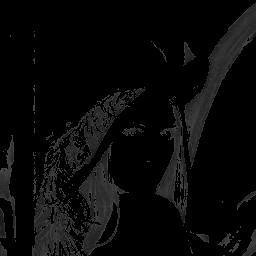
\includegraphics[scale=.8, clip]{img/02_region_01.jpg}
	\caption[]
  {Region pierwszy (z pięciu) po segmentacji.}
\end{figure}

\FloatBarrier

\begin{figure}[h!]
  \centering
  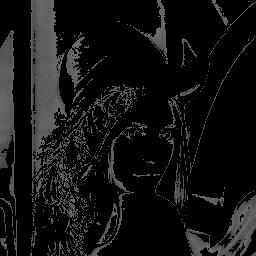
\includegraphics[scale=.8, clip]{img/02_region_02.jpg}
	\caption[]
  {Region drugi (z pięciu) po segmentacji.}
\end{figure}

\FloatBarrier

\begin{figure}[h!]
  \centering
  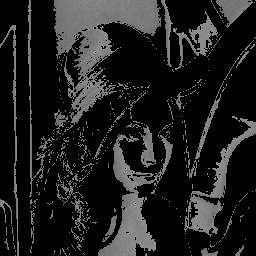
\includegraphics[scale=.8, clip]{img/02_region_03.jpg}
	\caption[]
  {Region trzeci (z pięciu) po segmentacji.}
\end{figure}

\FloatBarrier

\begin{figure}[h!]
  \centering
  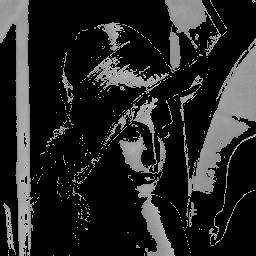
\includegraphics[scale=.8, clip]{img/02_region_04.jpg}
	\caption[]
  {Region czwarty (z pięciu) po segmentacji.}
\end{figure}

\FloatBarrier

\begin{figure}[h!]
  \centering
  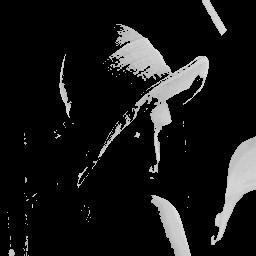
\includegraphics[scale=.8, clip]{img/02_region_05.jpg}
	\caption[]
  {Region piąty (z pięciu) po segmentacji.}
\end{figure}

\FloatBarrier

\end{document}